\documentclass[pdf]{beamer}
\usetheme{Copenhagen}
\usepackage{multicol, latexsym, amsmath, amssymb}
\usepackage{smartdiagram}
\usepackage{subcaption}

\setbeamertemplate{navigation symbols}{}
\newcommand{\z}{\mathbf{z}}
\newcommand{\uout}{u_{out}}
\newcommand{\vout}{v_{out}}
\newcommand{\uoutdum}{u_{out}^{dum}}
\newcommand{\uinplus}{u_{in}^{+}}
\newcommand{\uinminus}{u_{in}^{-}}
\newcommand{\winl}{w_{in}^{l}}
\newcommand{\win}{w_{in}}
\newcommand{\uin}{w_{in}}
\newcommand{\vin}{v_{in}}

\DeclareMathOperator*{\plusrightarrow}{\ensuremath{\xrightarrow{+}}}
\DeclareMathOperator*{\minusrightarrow}{\ensuremath{\xrightarrow{-}}}
\DeclareMathOperator*{\plusleftarrow}{\ensuremath{\xleftarrow{+}}}
\DeclareMathOperator*{\minusleftarrow}{\ensuremath{\xleftarrow{-}}}

\title{Meaning in Locke}
\subtitle[]{Meaning of Meaning Workshop}

\author{Ananth Mahadevan}
\date{\today}

\begin{document}
\begin{frame}
    \titlepage
\end{frame}

% \begin{frame}
%     \frametitle{Contents}
%     \tableofcontents
% \end{frame}


\section{Evaluation Pipeline}

\begin{frame}<1>[label=Pipeline]
  \frametitle{Pipeline Overview}
  
\begin{figure}
    \centering
    \tikzstyle{textblock} = [rectangle, text width=4em, text centered, line width=1pt]
\tikzstyle{block} = [rectangle, draw, fill=uablue25, 
    text width=5em, text centered, rounded corners, minimum height=2em, line width=1pt ]
\tikzstyle{line} = [line width=1pt, -triangle 45]
\tikzstyle{alert} = [text=uared100, fill=uared25, draw=uared100]
\tikzstyle{normal} = [text=uablue100, fill=uablue25, draw=uablue100]
\tikzstyle{dim} = [text=uablue25, fill=uablue5, draw=uablue25]
\tikzstyle{hide} = [draw=None]
\begin{tikzpicture}[node distance=1.5cm, auto]
    % Place nodes
    \node [block,onslide=<2->{dim}] (quote) {Find Locke Quotes};
    \node [block,onslide=<2->{dim},above right=2.5mm of quote] (blast)  {Get BLAST Hits};
    \node [block,onslide=<2->{dim},below right=2.5mm of quote] (sem)  {Get Semantic Search Hits};
    \node [block,onslide=<2->{dim}, right=2.5cm of quote] (sort) {Sort and Filter};
    
    \node [block,onslide=<2->{dim},temporal=<2>{}{alert}{dim}, above right=1cm of sort] (uniqblast) {Unique BLAST Hits};
    \node [block,onslide=<2->{dim}, right=1cm of sort] (intersection) {Intersection Hits};
    \node [block,onslide=<2->{dim},temporal=<3>{}{alert}{dim}, below right=1cm of sort] (uniqsem) {Unique Semantic Hits};
    
    \draw[line,onslide=<2->{dim}] (quote.north) -- (blast.west);
    \draw[line,onslide=<2->{dim}] (quote.south) -- (sem.west);
    
    \draw[line,onslide=<2->{dim}] (blast.east) -- (sort.north);
    \draw[line,onslide=<2->{dim}] (sem.east) -- (sort.south);

    \draw[line,onslide=<2->{dim}] (sort.east) -- (uniqblast.south west);
    \draw[line,onslide=<2->{dim}] (sort.east) -- (intersection.west);
    \draw[line,onslide=<2->{dim}] (sort.east) -- (uniqsem.north west);

\end{tikzpicture}
\end{figure}
\end{frame}


\againframe<2>{Pipeline}

\section{Unique BLAST Hits}
\begin{frame}
  \frametitle{Unique BLAST Hits}

  \begin{itemize}
    \item<3> Text reuse hits with lots of OCR noise
  \end{itemize}
  \only<1>{\begin{block}{Example John Locke Quote}
  ``The Animal and Vegetable Kingdoms are to nearly join'd, that if you will take the lowest of one, and the highest of the other, there will scarce be perceived any great difference between them.''
  \end{block}}
  \only<2->{\begin{block}{Example John Locke Quote Piece}
  ``the Animal and Vegetable Kingdoms, are so nearly join'd, that if you will take the lowest of one, and the highest of the other, there will scarce be perceived an''
  \end{block}
  }
  
  \begin{block}<3->{BLAST Hit}
    ``he Ani-\textbackslash{}nm Ial\textasciitilde{}andr Vegetable- KingdomsS are \textbraceleft{}ol\textasciitilde{}4 news\textasciitilde{}l \textbackslash{}' " \textbackslash{}'d, that if\textbackslash{}nyoul will takie the\textbackslash{}' lowes .of: one, and the ofp\textasciitilde{}\textasciitilde{}p the other,\textbackslash{}nthere will \textasciitilde{}fearce be perceived an''
  \end{block}

\end{frame}

\begin{frame}
  \frametitle{\href{https://gallica-kaiku.rahtiapp.fi/?eccoId=1702800107&offsetStart=357168&offsetEnd=357338}{Unique BLAST Hit Document}}
  \begin{figure}[]
    \centering
    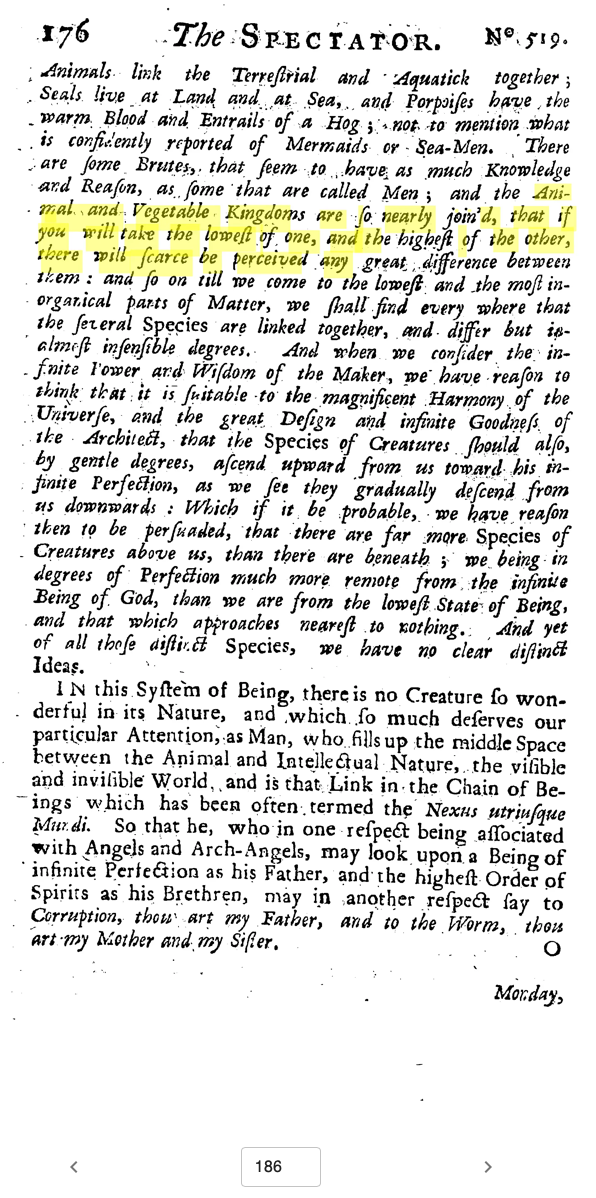
\includegraphics[width=\linewidth,height=\textheight,keepaspectratio]{images/blast_hit.png}
  \end{figure}
\end{frame}

\section{Unique Semantic Search Hits}

\againframe<3>{Pipeline}

\begin{frame}
  \frametitle{Unique Semantic Search Hits}
  \begin{itemize}
    \item Finds paraphrases and meaning matches
    \item Hits are always a fixed size of tokens
  \end{itemize}
  \begin{block}{Semantic Search Hit}
    ``in the vegetable and animal tribes belong-\textless{}br /\textgreater{}ing to the earth, and have discovered that the lowest of\textless{}br /\textgreater{}the animal species and the highest of the vegetable approx-\textless{}br /\textgreater{}imate so near to each other, that the difference betweenk\textless{}br /\textgreater{}the two can scarcely be perceived; but this is the very\textless{}br /\textgreater{}summit of their researches; they are unable to trace the\textless{}br /\textgreater{}connection of things any further, and reft satisfied in ad-\textless{}br /\textgreater{}mitting that\textless{}br /\textgreater{}\textless{}br /\textgreater{}The chain continues, but its''
  \end{block}
\end{frame}

\begin{frame}
  \frametitle{\href{https://gallica-kaiku.rahtiapp.fi/?eccoId=1015500300&offsetStart=715621&offsetEnd=716054}{Semantic Search Hit Document}}
  \begin{figure}
    \centering
    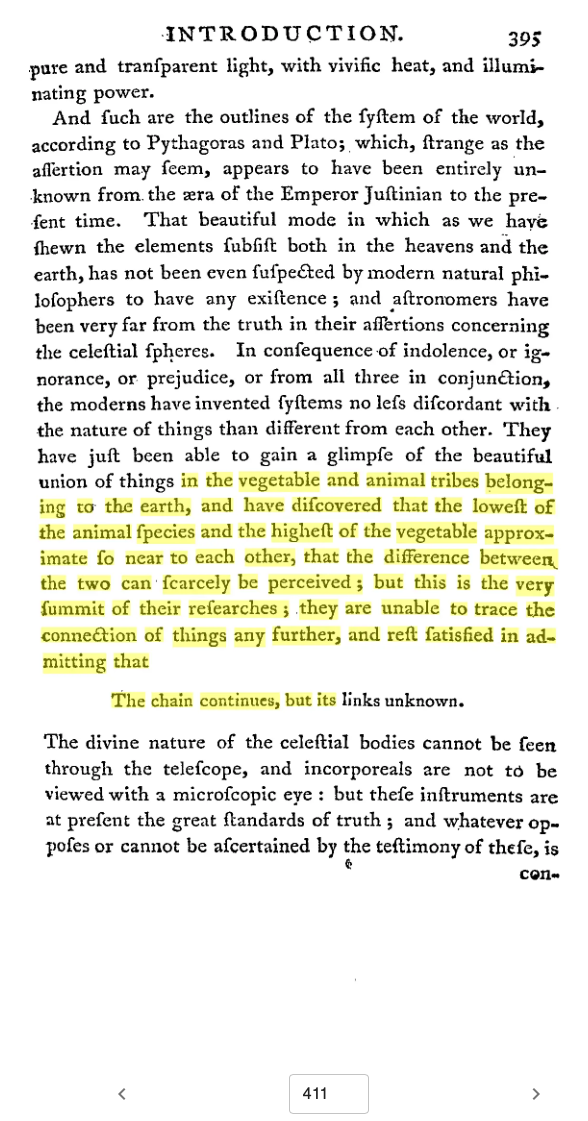
\includegraphics[width=\linewidth,height=\textheight,keepaspectratio]{images/semantic_hit.png}
  \end{figure}

\end{frame}


\section{Annotation}

\begin{frame}
  \frametitle{Annotation Pipeline}
  
\begin{figure}
    \centering
    \tikzstyle{textblock} = [rectangle, text width=4em, text centered, line width=1pt]
\tikzstyle{block} = [rectangle, draw, fill=uablue25, 
    text width=5em, text centered, rounded corners, minimum height=2em, line width=1pt ]
\tikzstyle{line} = [line width=1pt, -triangle 45]
\tikzstyle{alert} = [text=uared100, fill=uared25, draw=uared100]
\tikzstyle{normal} = [text=uablue100, fill=uablue25, draw=uablue100]
\tikzstyle{dim} = [text=uablue25, fill=uablue5, draw=uablue25]
\tikzstyle{hide} = [draw=None]
\begin{tikzpicture}[node distance=1.5cm, auto]
    % Place nodes
    \node [block,temporal=<2>{}{alert}{}] (quotes) {Sample Locke Quotes};
    \node [block,temporal=<3>{}{alert}{},right=0.7cm of quotes] (uniqsem) {Sample Unique Semantic Hits};
    \node [block,temporal=<4>{}{alert}{},right=0.7cm of uniqsem] (annotate) {Annotate};
    \node [block,temporal=<5>{}{alert}{},right=0.7cm of annotate] (eval) {Evaluate};
    \draw[line] (quote) edge (uniqsem) (uniqsem) edge (annotate) (annotate) edge (eval);


\end{tikzpicture}
\end{figure}
  \begin{itemize}
    \item<only@2> Sample 20 quotes from top 1000 quotes
    \item<only@3> Sample 50 after filtering 200K semantic hits
    \only<3>{\begin{enumerate}
      \item Group by \texttt{work\_id} and keep hit with highest certainty
      \item Top 5 hits
      \item 5 random hits from each 10\% interval
    \end{enumerate}}
    \item<only@4> Annotate with one of five options
    \only<4>{\begin{enumerate}
      \item Paraphrase 
      \item Meaning Match
      \item Topical
      \item No Match
      \item Don't Know
    \end{enumerate}
    }

  \end{itemize}
\end{frame}

\begin{frame}
  \frametitle{Annotation Results for example Locke quote}
  \begin{figure}
    \centering
    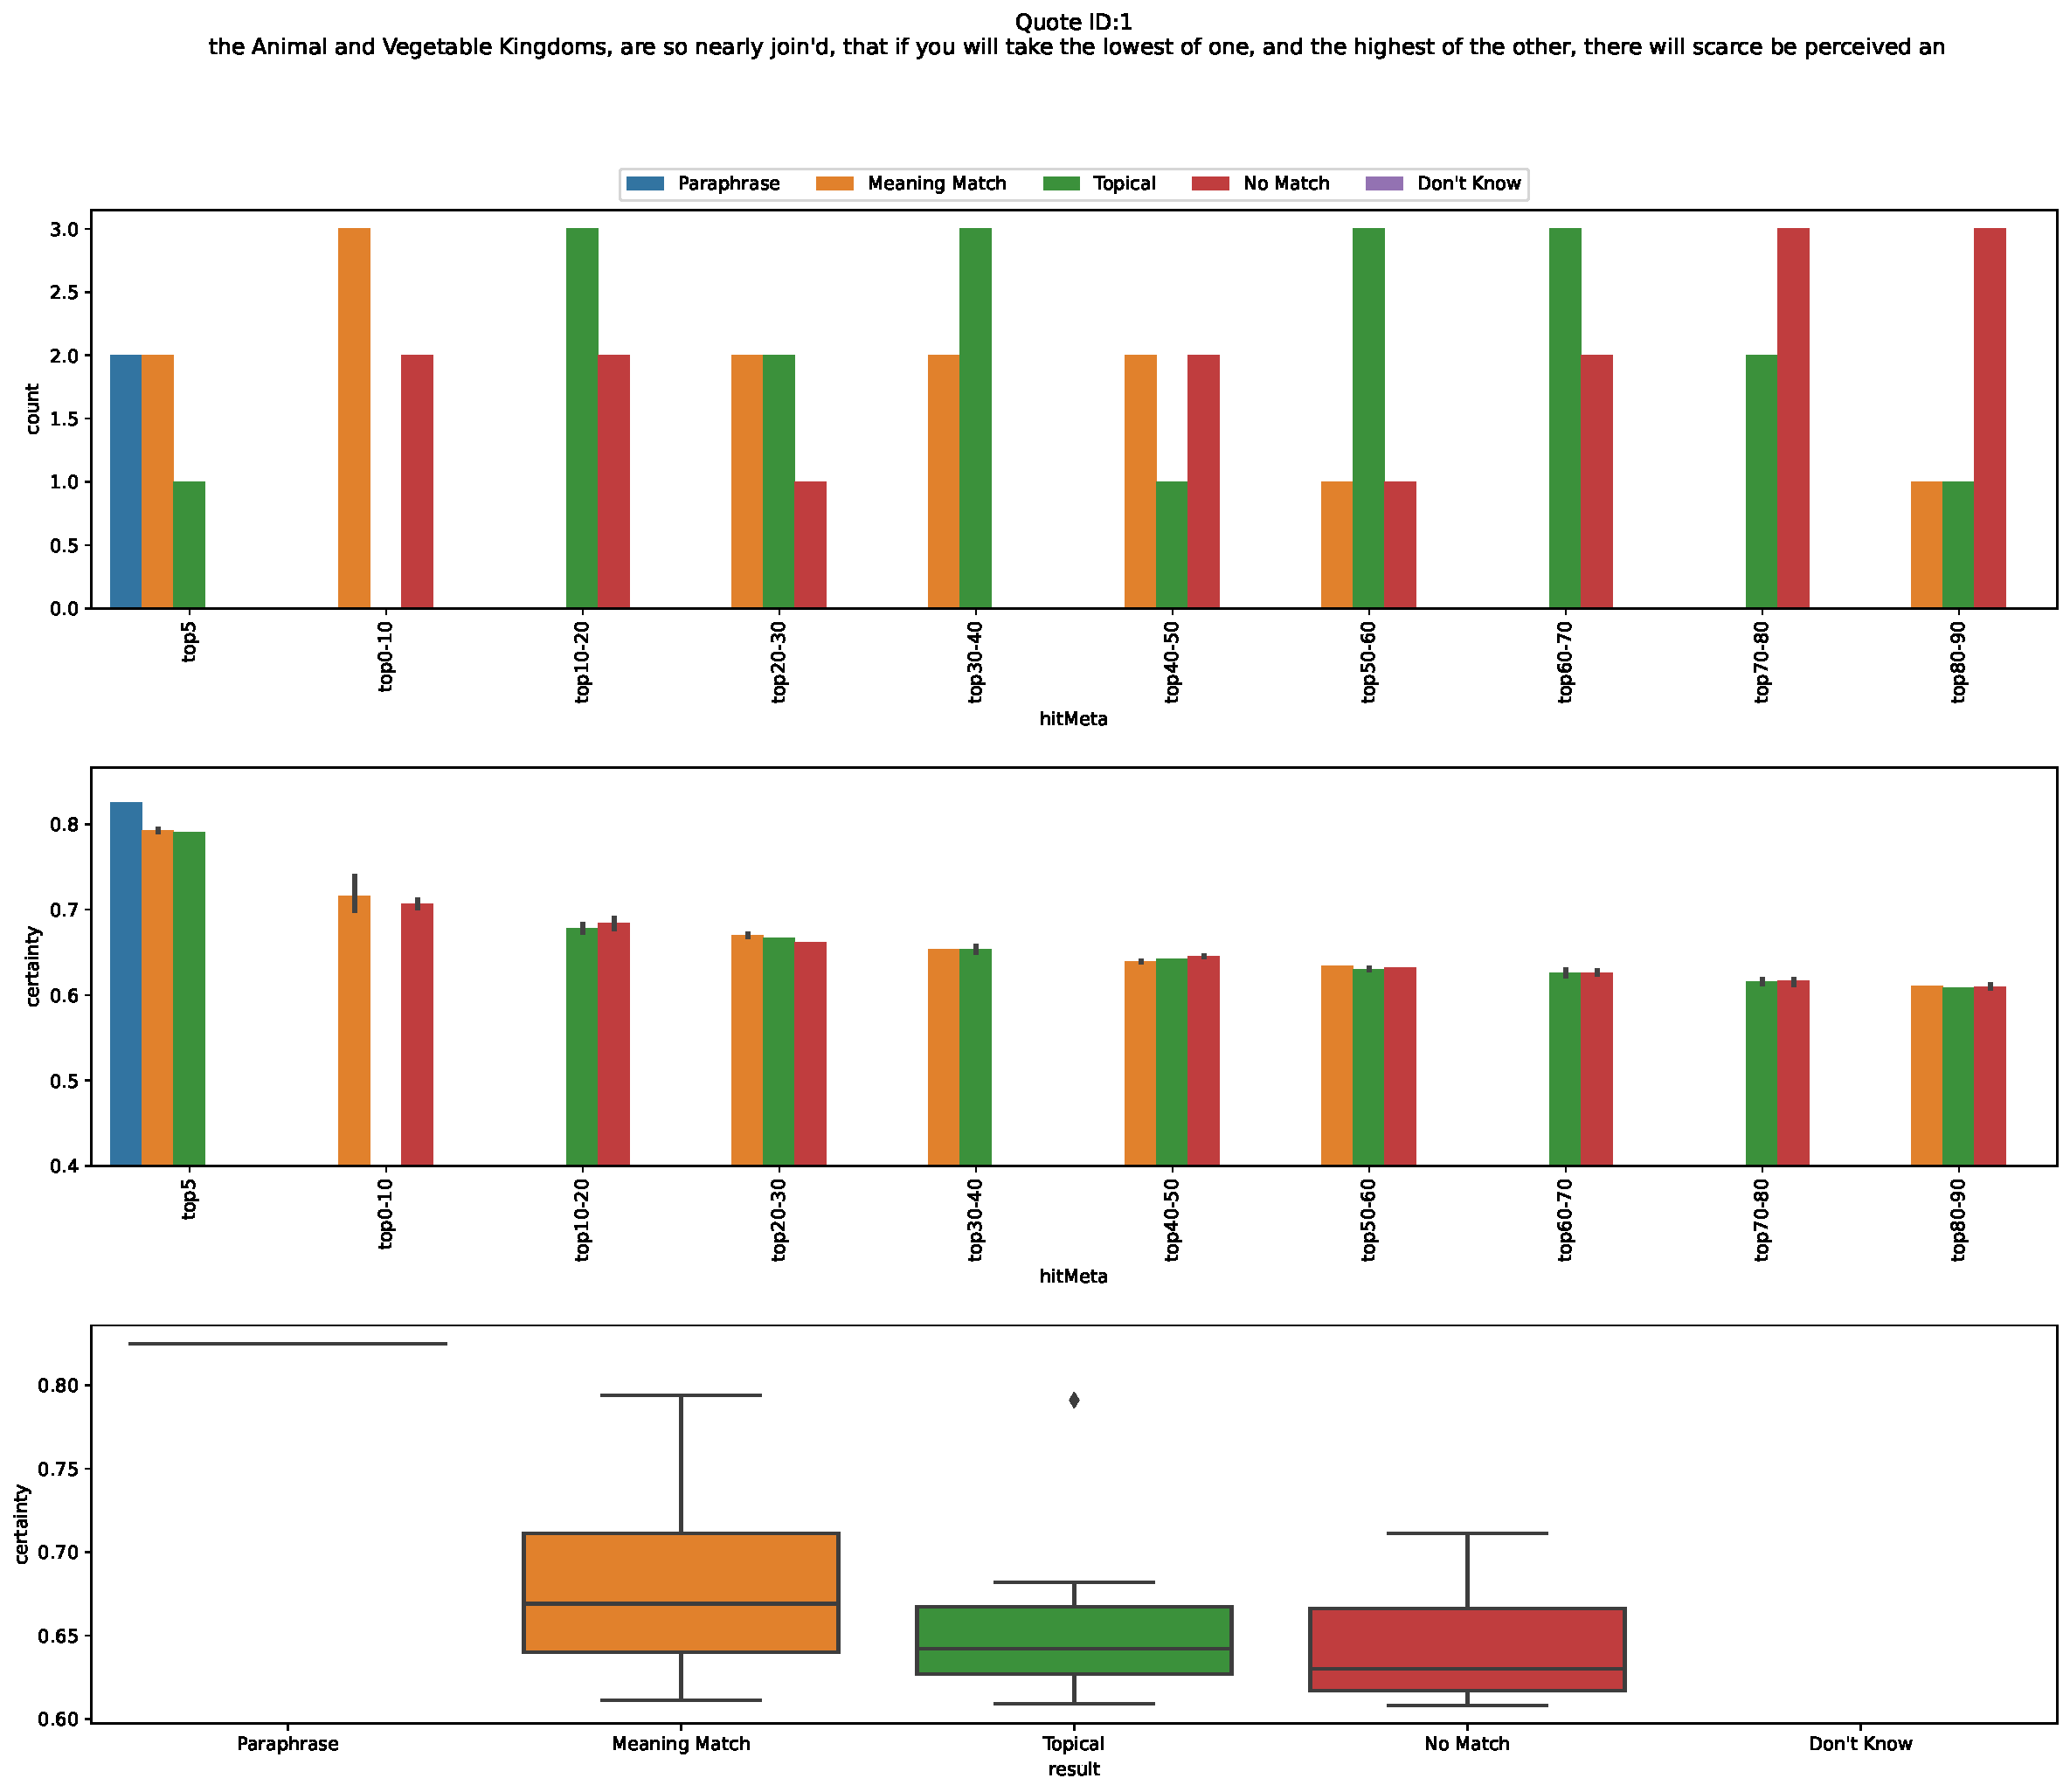
\includegraphics[width=\linewidth,height=\textheight,keepaspectratio,clip,trim={0 8cm 0 0}]{images/quote_1_annotation_results.pdf}
  \end{figure}
\end{frame}

\begin{frame}
  \frametitle{Meaning Match for Example Quote}
    \begin{figure}[htbp]
      \centering
      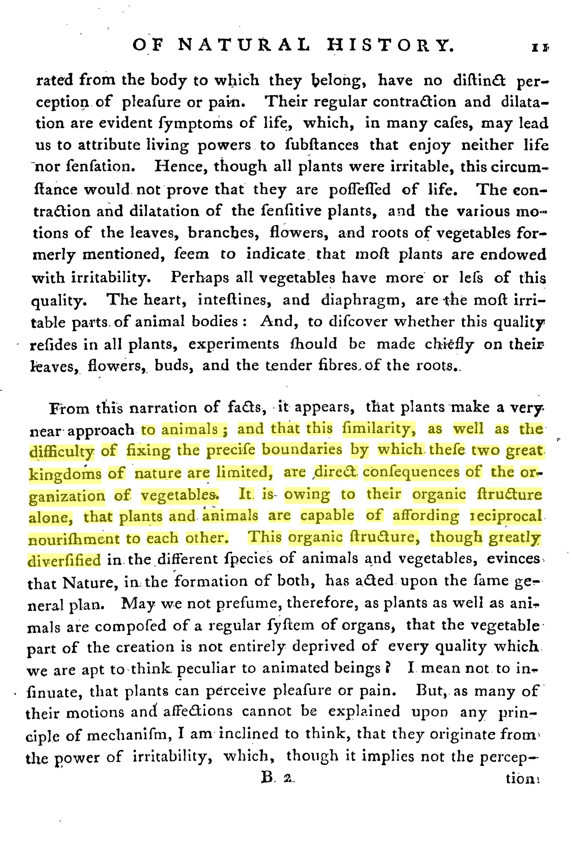
\includegraphics[width=\linewidth,height=\textheight,keepaspectratio]{images/meaning_match.png}
    \end{figure}
\end{frame}

\begin{frame}
  \frametitle{Topical Match for Example Quote}
  \begin{figure}[htbp]
    \centering
    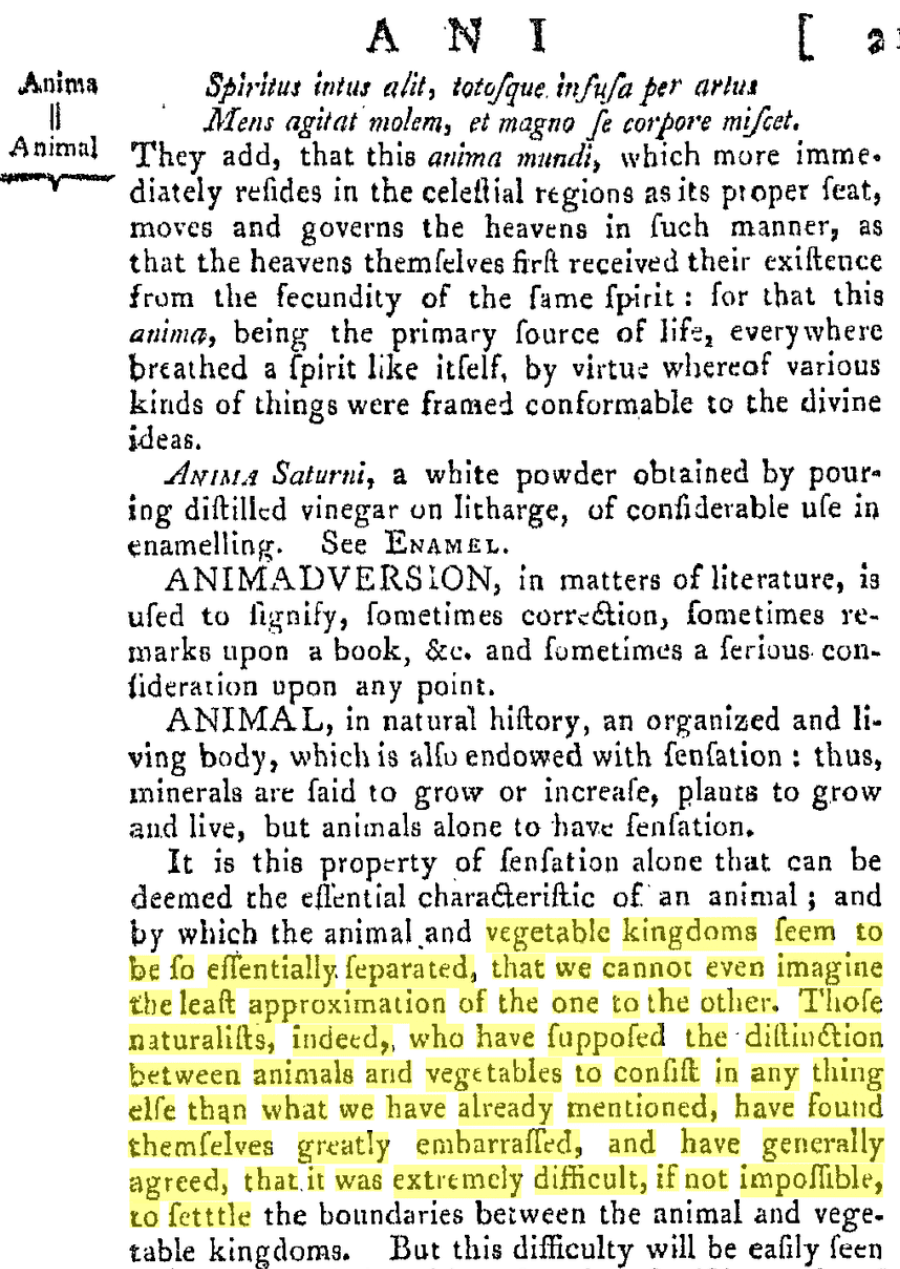
\includegraphics[width=\linewidth,height=0.8\textheight,keepaspectratio]{images/topical_match.png}
  \end{figure}

\end{frame}
\end{document}  